\textbf{\subsection{Расчет входного каскада}}
\vspace{1em}

Входной каскад выполнен на дифференциальном каскаде. Дифференциальный каскад характеризуется тем, что усиление по напряжению при симметричном съеме сигнала равен коэффициенту усиления в схеме с общим эмиттером. Как и предоконечный каскад, входной является усилителем по напряжению. Однако из-за ограниченного сопротивления в коллекторной цепи коэффициент усиления по напряжению дифференциального сигнала не будет достигать больших значений. При этом синфазный сигнал подавляется значительно, что является уменьшением синфазных помех. 
За счет отсутствия местной обратной связи в дифференциальном каскаде достигается большое увеличение по напряжению.  Что непосредственно влияет на петлю ООС в усилителе мощности, увеличивая коэффициент усиления в петле ООС.
Транзисторы VT1 и VT2 работают в режиме А, который обеспечивает усиление по напряжению, но не дает большого КПД.

\begin{figure}[!htbp]
    \center{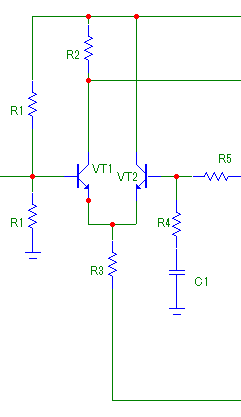
\includegraphics[width=0.23\linewidth]{picture_vh}}
    \caption{Схема входного каскада}
    \label{figure:p2_5}
  \end{figure}

VT1 и VT2 – дифференциальный каскад.
R1 – сопротивление базового делителя. Ограничивает входное сопротивление каскада.
R3 – сопротивление эмиттерной цепи.
R2 – сопротивление коллекторной цепи. Задает нагрузку каскада.
R5, R4 и C1 – цепь обратной связи. По постоянному току 100\%, по переменному определяется сопротивлением резистора R4.

\subsubsection{Ток покоя коллектора VT1 и VT2:}

\begin{equation}
\label{eq:equation4_1}
 I_{\text{0 К1}} = (5 \ldots 10) I_{\text{Б m3}} / h_{\text{21 3}} = 7 \cdot 0.024 / 80 = 2.1 ~ \text{мА} 
\end{equation}

\subsubsection{Параметры выбора транзисторов:}

\begin{equation}
\label{eq:equation4_1d}
 I_{\text{К1}} = (1.1 \ldots 1.3) I_{\text{0 К1}} = 1.1 \cdot 0.002 = 2.3~\text{мА}
\end{equation}
\begin{equation}
\label{eq:equation4_2}
f_{\text {h21}}=(5\ldots 10) f_{\text{в}}=8 \cdot 18000=144~\text{кГЦ}
\end{equation}

тут типо таблица ,но я их не умею делать априори

\subsubsection{Выбор сопротивления $R_{\text{2}}$:}
\begin{equation}
\label{eq:equation4_3}
R_2 = U_{\text{БЭ3}}/(I_{\text{0K1}}-I_{\text{0БЗ}})=(0.6 \ldots 0.7)/(0.0021-0.002/50)=338 ~\text{Ом}
\end{equation}

\subsubsection{Выбор сопротивления $R_{\text{3}}$:}

\begin{equation}
\label{eq:equation4_4}
R_3=\dfrac{E_{\text{0}}- U_{\text{БЭ}}} {2 \cdot I_{\text{0Э1}}} = \dfrac{E_{\text{0}}-U_{\text {БЭ1}}}{ 2 \cdot ( I_\text{0K1}+I_\text{0K1} / h_\text{21} )}
\end{equation}
\begin{equation*}
R_3=\dfrac{17-0.7}{ 2 \cdot(0.0021 + 0.0021 / 50)} = 3.80~\text{кОм}
\end{equation*}


\subsubsection {Цепь обратной связи :}

По обратной связи сигнал с выхода усилителя (точка соединения RH) подается на переход БЭ первого транзистора. При этом следует учитывать, что внутреннее сопротивление дифференциального каскада равно 2h11. Передача сигнала по ООС будет производиться по цепи обратной связи R5, R4 и C1.


\begin{equation}
\label{eq:equation4_5}
\beta = [\dfrac {R_{\text{ЭКВ}}}{R_{5}+R_{\text{ЭКВ}}}] \cdot [\dfrac {r_{\text{БЭ1}}}{R}]=306/(5000+306) \cdot (600/3356)=0.0103
\end{equation}

\begin{equation}
\label{eq:equation4_6}
R=2 \cdot h_{11}+R_{\text{ЭГ}}=2 \cdot h_{11}+R_1 \cdot 2 \cdot h_{11}+\dfrac{R_1 \cdot R_{\text{Г}}}{(R_1+R_{\text{Э}})}=2 \cdot h_{11}+R_{\text{ЭГ}}
\end{equation}
\begin{equation*}
R=2 \cdot 11 +3333=3356~\text{Ом}
\end{equation*}

Сопротивление RЭГ является сопротивлением между базой транзистора VT1-VT2 и землей по переменному току. При расчете RЭГ необходимо руководствоваться следующими соображениями:
\begin{equation}
\label{eq:equation4_7}
R_{\text{ЭГ}}=\dfrac{R_1 \cdot R_{\text{Г}}}{R_1+R_{\text{Г}}}=5000 \cdot 10000 / (5000 + 10000) = 3333~\text{Ом}
\end{equation}

При этом RГ – выходное сопротивление каскада предварительного усиления, выполненного по схеме эмиттерного повторителя. Входное сопротивление этого усилителя имеет большую величину, выходное относительно малую порядка сотен Ом и зависит от сопротивления выходного регулятора тембра, который имеет большое входное сопротивление, порядка тысяч Ом.
Для того чтобы сопротивление R1, включенное параллельно RГ, существенно не влияло на сопротивление генератора, примем его равным порядка кила Ом:

\begin{equation}
\label{eq:equation4_8}
R_1= 5~\text{кОм и }~R_{\text{Г}} = 3000 ~\text{Ом} 
\end{equation}
\begin{equation}
\label{eq:equation4_9}
h_{\text{11}}=\dfrac{(1+h_{\text{21}}) \cdot \psi_{\text{Т}}}{  I_{\text{0 Э1}}} = (1+50)\cdot 0.025 / 0.002 =607~\text{Ом}
\end{equation}
\begin{equation}
\label{eq:equation4_10}
R_{\text {ЭКВ}}=R_4 \cdot R / (R_4+R)=336 \cdot 3356 / (336+3356)=306~\text{Ом}
\end{equation}
Для сохранения идентичности режимов VT1 и VT2 сопротивление R1 выбирается равным R5. R5 выбираем из ряда:
\begin{equation}
\label{eq:equation4_11}
R_{\text{5}}=(20 \ldots 100) \cdot R_{\text{Н}}=100 \cdot 2 = 200~\text{Ом}
\end{equation}
\begin{equation}
\label{eq:equation4_12}
R_{\text{5}}=5000~\text{Ом}
\end{equation}

\begin{equation}
\label{eq:equation4_13}
R_4=\dfrac{(F-1) \cdot R \cdot R_5}{h_{\text{21}} \cdot R_{\text{КН1}} \cdot K_{\text{ПОК}}-(F-1)\cdot (R+R_{\text{5}})}
\end{equation}
\begin{equation*}
R_4 = 24 \cdot 3356 \cdot 5000 / (50 \cdot 44 \cdot 631 -24 \cdot 8356)=336~\text{Ом}
\end{equation*}

\begin{equation}
\label{eq:equation4_14}
R_{\text{КН1}}=\dfrac{R_2 \cdot R_{\text{ВХ3}}}{ R_{\text{2}}+R_{\text{ВХ3}}}=338 \cdot 51/ (338+51)=44~\text{Ом}
\end{equation}

Отношение R4  к R5 характеризует ООС по переменному току. За счет сопротивления R4 по переменному току обратная связь не 100\%, но за счет малости R4 имеет величину порядка 95\%.
Значение F выбирается из предварительного расчета: F = 25
Коэффициент петлевого усиления:

\begin{equation}
\label{eq:equation4_15}
K_{\text{П}}=\beta \cdot K_{\text{ВК}} \cdot K_{\text{ПОК}} \cdot K_{\text{OK}}=0.0103 \cdot 3.7 \cdot 631 \cdot 1 =24
\end{equation}

\begin{equation}
\label{eq:equation4_16}
K_{\text{ВК}}=S_1 \cdot R_{\text{КН1}}=\dfrac{R_{\text{КН1}}}{r_{\text{Э}}}=44 \cdot 0.0021/0.0025=3.7
\end{equation}

\begin{equation}
\label{eq:equation4_17}
K_{\text{ОК}}=1
\end{equation}

Входное сопротивление усилителя:

\begin{equation}
\label{eq:equation4_18}
R_{\text{ВХВК}}=\dfrac{R_1 \cdot (2 h_{11}+R_4) \cdot F}{R_1+(2 \cdot h_{11}+R_{\text{4}}) \cdot F} 
\end{equation}
\begin{equation*}
R_{\text{ВХВК}}= 5000 \cdot(2 \cdot 607+336) \cdot 25 / (5000+(2 \cdot 607+336) \cdot 25)=4429~\text{Ом}
\end{equation*}

Конденсатор C2 служит для устранения возможности самовозбуждения на высоких частотах:

\begin{equation}
\label{eq:equation4_19}
C_2=\dfrac{R_{\text{2}}+R_{\text{ВХ3}}}{2 \cdot \pi f_{\text{в}} K_{\text{ПОК}} \cdot R_2 \cdot R_{ВХ3} }=(338+51)/(2 \cdot 3.142 \cdot 18000 \cdot 631 \cdot 4 \cdot 338)=83~\text{пФ}
\end{equation}

\subsubsection{Выбор емкости C1:}

Эта емкость устраняет 100\% обратную связь по переменному току.
\begin{equation}
\label{eq:equation4_20}
C_1=\dfrac{1}{2 \cdot \pi\cdot f_{\text{н}} \cdot R_4 \cdot \sqrt{M^2-1}}=1/[2 \cdot 3.14 \cdot 10 \cdot 336 \cdot \sqrt{3.00^2-1}]=16.7~\text{мкФ}
\end{equation}

\subsubsection{	Коэффициент требуемого усиления по напряжению рассчитанного усилителя мощности:}

\begin{equation}
\label{eq:equation4_21}
K_{\text{УМ}}=\dfrac{1}{\beta}=1/0.0103=97.1
\end{equation}

Также усиление по напряжению каскада усиления мощности можно определить через глубину обратной связи:

\begin{equation}
\label{eq:equation4_22}
K_{\text{УМ}}=\dfrac {K_{\text{Е}}}{K_{\text{УМ}}}=3.46/171=0.02~\text{В}
\end{equation}

\subsubsection{Требуемое входное напряжение при номинальной выходной мощности:} % (fold)


\begin{equation}
\label{eq:equation4_23}
U_{\text{ВХВК}}=\dfrac{U_{\text{Н}}}{K_{\text{УМ}}}=5.657/97.07=0.06 ~\text{В}
\end{equation}

Сопротивление дифференциального каскада ограничивается сопротивлениями базового делителя R1 и сопротивление источника сигнала, каковым для него является КПУ 2, выполненный по схеме с ОК, выходное сопротивление которого имеет небольшую величину.
\subsubsection{	Итоговые данные предоконечного каскада:	}

\begin{table}[htbp]
\caption{Параметры выбора транзистора}
\begin{center}\begin{tabular}{|c|c|c|c|c|c|c|}
\hline 
  & тип & $P_{\text{к}}$ доп, Вт & $I_{\text{к}}$ доп, А & $U_{\text{к}}$ доп, В & $h_{21}$ &  $f_{h_{21}}$, кГц \\ 
\hline 
VT1/2 & n-p-n & 3.66  & 3.11 & 19 & 400 & 36.00\\ 
\hline 
\end{tabular} 
\end{center}
\end{table}

\clearpage

\begin{table}[htbp]
\caption{Режимы работы транзистора}
\begin{center}\begin{tabular}{|c|c|c|c|c|c|c|c|c|c|c|c|c|}
\hline 
   & $I_\text{0К}$ & $I_\text{0б}$& $U_\text{0Б}$ & $U_\text{0К}$&  $I_{\text{Км}}$  & $I_{\text{Бм}}$& $U_{\text{км}}$, B & $P_{\text{к}}$ & K\\ 
  & мА & мА& В & В & мА & мА & B & мВт & \\
\hline 
КТ127А-1 & 1 & 0.03 & 0.7 & 5 & 50 & 1.66 & 25 & 15 & 0.99 \\
\hline
\end{tabular} 
\end{center}
\end{table}